\chapter{Proof of concept: Interacting with Excel documents with Microsoft Graph} % Main chapter title

\label{Proof of concept1} % Change X to a consecutive number; for referencing this chapter elsewhere, use \ref{ChapterX}

%----------------------------------------------------------------------------------------
%	SECTION 1
%----------------------------------------------------------------------------------------

\section{App registration and permission granting on the Azure Portal}

Below it can be seen how the app registration process looks like on the Azure Portal. There needs to be an app name defined as well as supported account types. Also there can optionally be an redirect URI defined where the authentication response goes to after a successful authentication \cite{MSAppReg}. 

\begin{figure}[h!]
  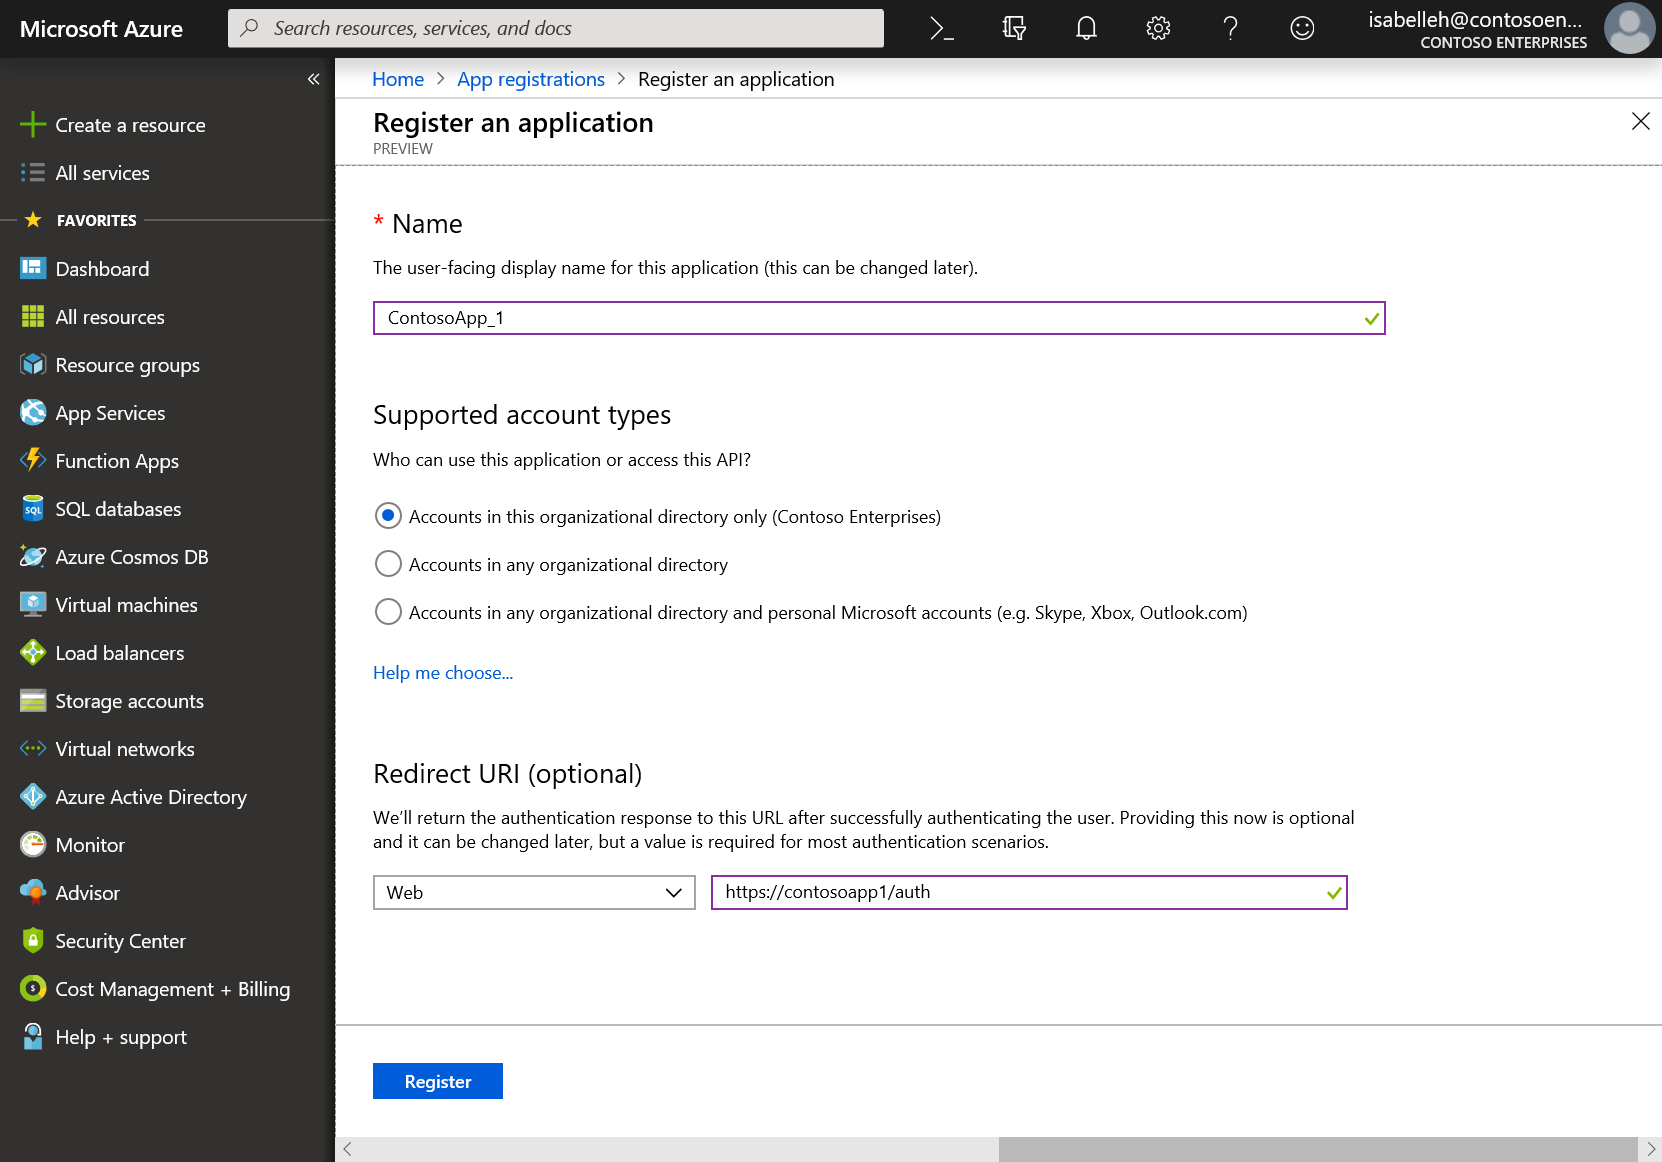
\includegraphics[scale=0.45]{Figures/new-app-registration-expanded.png}
  \caption{App registration process}
  \label{fig:App registration process}
\end{figure}

For the web-app to be created it makes sense to use client credentials authentication provider, as it is favourable to have authentication without user interaction. In that case a Share-point online (SPO) license is required in order to use the Graph. Such a license is only available in work or school accounts. Attempts with a private account and an Office 365 subscription failed, as for private accounts its not possible to have an SPO license. As at ZHAW, the use of Graph is restricted by System admins, such an admin needs to be contacted. The system admin has to create a test user, assign the required SPO license to that test user and register the application. 

The system admin is further required to create a client secret as shown below. The application uses to client secret to authenticate at the Microsoft Identity Platform.

\begin{figure}[h!]
  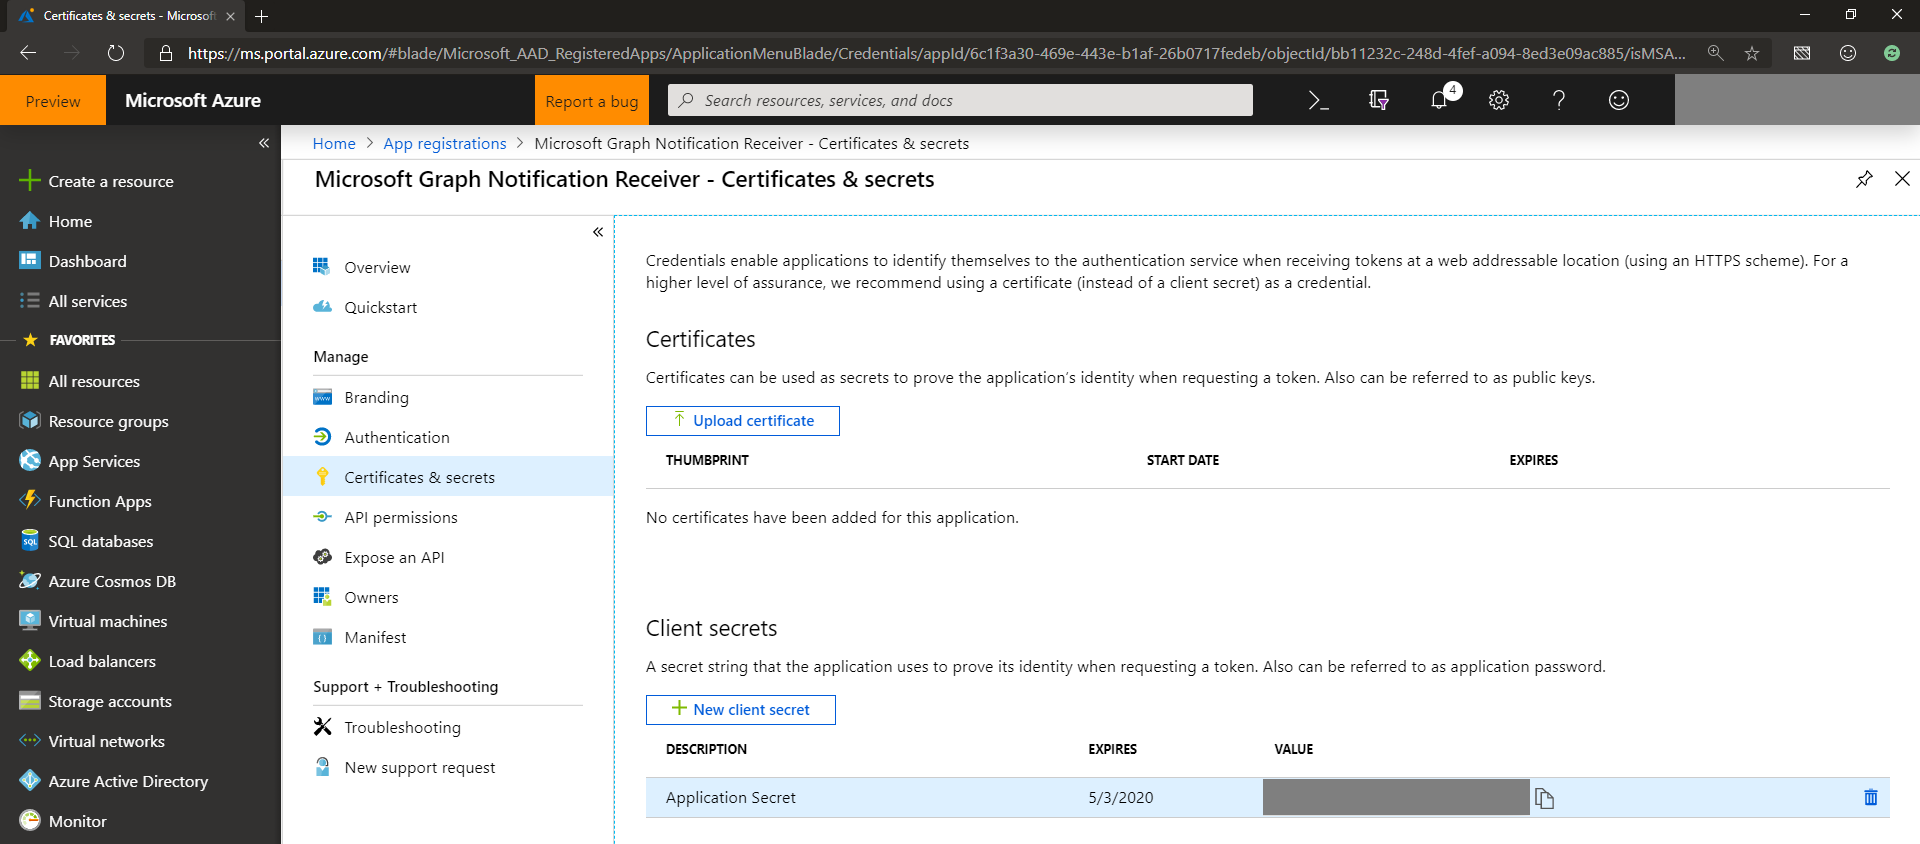
\includegraphics[scale=0.275]{Figures/client-secret.png}
  \caption{Client secret}
  \label{fig:Creation of client secret}
\end{figure}

Also, the API permissions need to be defined in the app, so they can be written to the access token which is needed for every http request. This can be done in the "API permission section" as shown as below:

\begin{figure}[h!]
  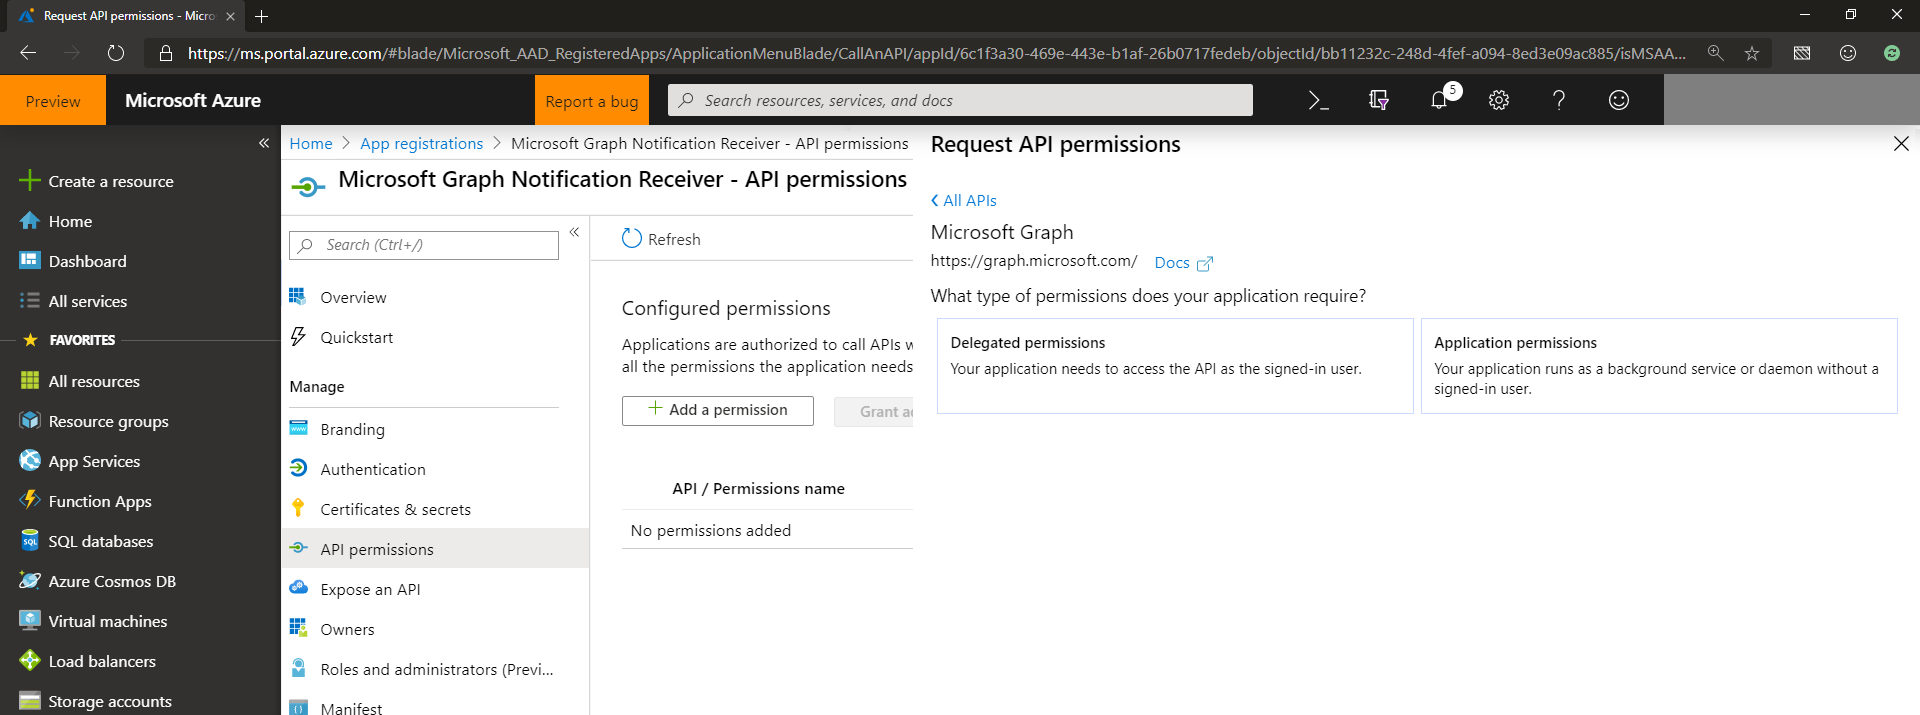
\includegraphics[scale=0.275]{Figures/notifications-api-permissions.png}
  \caption{API permissions}
  \label{fig: Adding API permissions}
\end{figure}

Following API permissions need to be selected in order to access the Excel document. The permission also need to be consented by the system admin:


\begin{longtable}[]{@{}lll@{}}
\toprule
Permission Name & Type & Description\tabularnewline
\midrule
\endhead
Access.Review.ReadWrite.All & Application & Manage all access reviews\tabularnewline
Directory.Read.All & Application & Read directory data\tabularnewline
Files.ReadWrite.All & Application & Read and write files in all site collections\tabularnewline
Sites.Read.All & Application & Read items in all site collections\tabularnewline
User.Read & Delegated & Sign in and read user profile\tabularnewline
User.Read.All & Application & Read all users' full profile\tabularnewline
\bottomrule
\caption{Required API permissions}
\label{Required API permissions}
\end{longtable}

After the application registration has been completed, the program to interact with the Excel document can be implemented. In the code snippet below from the Microsoft documentation it can be seen that, the client credentials flow requires that you request the default scope. Further, the respective values and ID's from the Azure portal need to be replaced with the according placeholders. Using the Azure.Idenity package, the client crendetials authorisation provider can be used to handle the process of access token aquisition. The access token is used in following for every API call made by the programme. API requests can be with the use of the graphCLient object which needs to be initiated.



\begin{lstlisting}[escapeinside={(*}{*)}, numbers=left]

var scopes = new[] { "https://graph.microsoft.com/.default" };

var tenantId = "common";

var clientId = "YOUR_CLIENT_ID";
var clientSecret = "YOUR_CLIENT_SECRET";

// using Azure.Identity;
var options = new TokenCredentialOptions
{
    AuthorityHost = AzureAuthorityHosts.AzurePublicCloud
};

// https://docs.microsoft.com/dotnet/api/azure.identity.clientsecretcredential
var clientSecretCredential = new ClientSecretCredential(
    tenantId, clientId, clientSecret, options);
    
var graphClient = new GraphServiceClient(clientSecretCredential, scopes);
} 
\end{lstlisting}\\

When further adding the below code to the programme, an Http get request will be triggered to read a cell from a sample Excel document. In the example shown, an Http request will be sent to the Graph API which returns the content of cell D53 in a JSON file.  


\begin{lstlisting}[escapeinside={(*}{*)}, numbers=left]
WorkbookRange range = await graphClient.Users["fd82005b-9ac2-4a48-ad36-e79cf3c366c7"]
                .Drive.Items["01SZPLU2I7EUC7NJFOKJA3QWJLZ2I74CEA"]
                .Workbook
                .Worksheets["Arbeit"]
                .Cell(54, 4)
                .Request()
                .GetAsync();
\end{lstlisting}\\

Furthermore the below code snippet can be used to write data into a cell of the same sample Excel document. In order to do so, the value must at first be parsed to a JsonDocument and saved to a WorkbookRange object so it can be sent along with an Http put request. 

\begin{lstlisting}[escapeinside={(*}{*)}, numbers=left]
var a = JsonDocument.Parse(@"""Frank Lampard""");

           
WorkbookRange nRange = new WorkbookRange();
nRange.Values = a;


await graphClient.Users["fd82005b-9ac2-4a48-ad36-e79cf3c366c7"]
                .Drive.Items["01SZPLU2I7EUC7NJFOKJA3QWJLZ2I74CEA"]
                .Workbook
                .Worksheets["Arbeit"]                
                .Range("A27")
                .Request()
                .PatchAsync(nRange);
\end{lstlisting}\\
